\documentclass[a4paper]{report}
\usepackage{sentivent}
%use \tagged{full}{text} to have extra text for full publication with academic details, not relevant for students.
\usetag{meta}

\addbibresource{references.bib}

\title{
    
\includegraphics[width=5cm]{img/sentiventlogo-gradient.png}\\
    [10pt]{\huge\bfseries {\Huge S{\huge ENT}i{\huge VENT}}\\
    Sentiment Annotation Guidelines\\
    v\vhCurrentVersion\\
    \Large{\normalfont{Technical Report}}
    }
}
\author{Gilles~Jacobs \\ \small{\texttt{gillesm.jacobs@ugent.be; gilles@jacobsgill.es}}}
\date{February 2020}

\begin{document}

\tagged{full}{
\maketitle
\tableofcontents
\newpage


\begin{versionhistory}
  \vhEntry{0.1}{28.02.2020}{{Gilles~Jacobs}}{Create initial draft with design choices and options.}
  \vhEntry{0.2}{09.03.2020}{{Gilles Jacobs}}{Implemented prototype annotation tools in WebAnno. Performed test annotations on aal00, aal01, aal02, aapl. Describe practical Guidelines.}
  \vhEntry{0.3}{05.04.2020}{{Gilles Jacobs}}{Added screenshots. Interface and workflow diagram figures.}
  \vhEntry{0.4}{08.04.2020}{{Gilles Jacobs}}{Performed annotation test on 15 different docs with colleagues (Joke Daems, Cynthia Van Hee, Margot Fonteyne Ayla Rigouts Terryn). Collect feedback and made following changes: Fix several typo's. Add ``difficult cases'' section. Conceptually unified sentiment annotations and events so that all same rules apply. Edit definitions to be more clear.}
  \vhEntry{0.5}{13.04.2020}{{Gilles Jacobs}}{Remove ``Conflict'' polarity label as it occurs very rarely: ``Conflict'' occurred 0 times across 15 documents in annotation testing and appeared only in 2\% of cases in EventDNA.}
  \vhEntry{0.6}{15.04.2020}{{Gilles Jacobs}}{Add ``notes'' with special cases.}
  \vhEntry{0.7}{21.04.2020}{{Gilles Jacobs}}{Add no more edge cases. }
  \vhEntry{0.9}{27.04.2020}{{Gilles Jacobs}}{Fixed final typo's and lay-out. Start annotation.}
  \vhEntry{1.0}{29.04.2020}{{Gilles Jacobs}}{Added note on Relevancy and added edga case for double events. Final version for annotation project.}
\end{versionhistory}
\label{chapter/rev}
}

\chapter{SENTiVENT Sentiment Guidelines} % change back to Introduction
\label{chapter/intro}
The \scheme codifies the annotation of sentiment in economic news articles.
Every news article contains news events communicating what is happening to companies such as a CEO change, a stock rating upgrade, analyst recommendations, a strike, the merger of two companies, etc.
The goal of \project is to automatically extract facts and opinions in a fine-grained manner from economic news.
Annotators will produce common-sense sentiment labels for economic events that will serve as training data to learn machine learning algorithms to extract this data/information automatically from text.

\tagged{full}{
\section{\project Goals and Task}
The goal of this annotation scheme is to produce a gold-standard labeled dataset for enabling aspect-based sentiment analysis in company-specific news.
The goal of the \project research project is to enable supervised learning for event extraction and sentiment analysis for economic news.
This requires a manually created gold standard dataset.
For the purposes of \project, an event in the business news-wire text domain are real-world occurrences that affect and involve companies.
The primary goal of company-specific news is reporting changes in the current state-of-affairs regarding businesses and the economy and associating that factual information with opinion data.
This is why automated sentiment analysis is a natural task for information extraction in this domain.
}

\section{Common-Sense Investor Sentiment}
\label{sec:sentimentdef}
An investor is someone looking to give capital to a company, product or asset with the expectation of profit in the future.
Investing is the act of allocating funds to an asset or committing capital to an endeavor (a business, project, real estate, etc.), with the expectation of generating an income or profit.
Sentiment are the attitudes and opinions a person holds towards a certain topic.
Investor sentiment then is the opinions that an investor holds towards a potential investee.
Generally, positive investor expectations come from events that have a desirable effect on a business entity's characteristics (e.g., its financial metrics, growth, position in the market) or the larger surrounding economic situation (e.g., macro-economic factors, policy changes, market fluctuations).
Examples of positive events are increases in growth of sales, revenue, profit, cash flow or other financial metrics, strategic investments, cut expenses, well-reviewed products, effective marketing efforts, growing stock price or increased price targets, upgraded ratings, optimistic analyst expectations, etc.

Negative investor sentiment entails the opposite expectation that a loss will be made and the invested funds will not be recuperated.
Generally, negative expectations come from events that have an undesirable effect on some attribute or the surrounding situation of a business entity.
Examples could be inhibition of growth/decline in sales, revenue, profit, cash flow and other financial metrics, or scandals, losses, legal issues, decreased expenses, lowering stock price or price targets, downgrading of ratings, employment issues, negative analyst expectations, etc.

\textbf{The type of subjective sentiment annotation we wish to annotate is of a prototypical investor who expects a return on investment.
}

\tagged{meta}{
\section{Practical Instructions on Annotation and Article Content}

\begin{itemize}[noitemsep, leftmargin=*]
    \item We encourage annotators to use search engines when they need to know more about a specific topic, company, ticker symbol, term, or other topics being discussed. Subsection \ref{subsec:resources} contains suggestions for economics and finance resources for information look-up.
    \item Annotators should at all times highlight any doubts regarding the annotation scheme and ask the supervisor for clarification. There are no stupid questions!
    \item Keep the guidelines handy during annotation and familiarize yourself thoroughly with the guidelines properly before beginning.
    \item The first line of the article is always the title. We annotate the title as we would the body.
    \item Annotators should advice the supervisor any issues and problems with the annotation tool and/or text on the team communications channel (Slack).
    \item Sentences that have no final punctuation but are followed by a full sentences are highly likely section titles of the article. These need to be annotated too.
\end{itemize}

\subsection{Webtools Used in Annotation}

\begin{itemize}[leftmargin=*]

    \item Video conferencing Jitsi Meet: For training annotators in voice/videochat environment. Open preferably in Chrome browser.\\
        \texttt{url: \url{https://meet.jit.si/lt3anno}}
    
    \item Video tutorial for annotator training. Annotators can follow along with the DEMO project on \url{https://webanno.lt3.ugent.be}:
    \begin{itemize}
        \item Part 1: \url{https://youtu.be/dHUj5vIOs68}
        \item Part 2: \url{https://youtu.be/alZmKXN2b3U}
    \end{itemize}

    \item Google Form for collecting annotator info:\\
        This form is to be filled by all annotators for the purpose of academic reporting on annotation quality. All data collected remains confidential, anonymous, and is not to be published.\\
        \texttt{url: \url{https://goo.gl/forms/0ZZvA6nG4pWQJlle2}}
    
    \item Annotation tool WebAnno v4.6.4:\\
        WebAnno is the annotation web tool in which all annotation work will be done.
        Use Chrome Browser to run WebAnno.\\
        \texttt{url: \url{http://webanno.lt3.ugent.be/}}\\
        \texttt{username: firstnamelastname}\\
        \texttt{password: lt34nn0}
        
    \item Collaboration channel Slack:\\
        Slack is an online chat-based collaboration environment for announcing issues in the annotation process and resolving annotation uncertainties. Annotators are to make an account before beginning annotation using their institutional email address.\\
        \texttt{url: \url{https://lt3anno.slack.com/}}\\
        
        Here you can discuss uncertainties and report any annotation issues.
\end{itemize}

\subsection{Information Sources}
\label{subsec:resources}
For an overview of a company or corporation, all of its subsidiaries (daughter companies) can be found at:

For general terminology, we advise to use a general purpose search engine.
Prioritize Wikipedia and Investopedia results.\\

\noindent
Glossaries explaining economic, financial, and investing terminology:
\begin{itemize}[noitemsep, leftmargin=*]
    \item Brief, recommended reading:\\ \url{https://am.jpmorgan.com/us/en/asset-management/gim/adv/glossary-of-investment-terms}
    \item \url{https://www.theguardian.com/business/glossary-business-terms-a-z-jargon}
    \item Investopedia dictionary (extensive): \url{https://www.investopedia.com/dictionary/}
    \item Financial Times Lexicon: \url{http://lexicon.ft.com/}
\end{itemize}

\noindent
Wikis for economics and finance:
\begin{itemize}[noitemsep, leftmargin=*]
    \item Investopedia contains a vast curated resource of financial knowledge. Use it:\\
    \url{https://www.investopedia.com/search/}
\end{itemize}

}

\chapter{Annotation Definitions}
\label{chapter/definitions}
% \section{The WebAnno interface}
% - show annotation panel
% - show sidepanel
% - clear
% - Explain existing annotations: What came before

\section{Sentiment Expression}
\label{sec:sentimentexpressiondefinition}
Sentiment can be both explicit expressions of opinion in the text as well as descriptions of events or situations with a specific connotation that evokes a certain sentiment.
\\\\
\noindent
A \textbf{Sentiment Expression is (sequence of) word(s)} that
\begin{enumerate}[label=\alph*), leftmargin=*]
    \item \textbf{affects \hyperref[sec:sentimentdef]{investor sentiment}} towards a company, market, stock, asset or person. e.g., \textit{``fall in stock price'', ``decline in sales and revenue'', ``increase in performance'', ``positive return on investment'', ``growing consumer interest''}.
    \item expresses positive or negative \textbf{opinion}. e.g. \textit{``strong performance'', ``being bad for'', ``fall from grace''}.
\end{enumerate}
\noindent
Look for words that stand out in conveying the content that would inform an investor’s opinion on a stock, person, market. Are there words that will influence the opinion of a potential investor?
It is likely that there are \textbf{multiple Sentiment Expressions per sentence}.
\textbf{Some Sentiment Expressions are already annotated as pre-existing Event annotations}.
You do not have to annotate new sentiment expressions on top of these Events.\\\\
\noindent
\textcolor{BrickRed}{NOTE: Avoid annotating full clauses: often annotating only the verb or the noun is sufficient for capturing the core meaning of the sentiment. Avoid annotating the companies, markets, stocks, assets or persons involved in the Sentiment Expression. Keep the \textbf{number of words as small as possible}.}

\begin{figure}[h]
    \centering
    
\includegraphics[width=\textwidth]{img/cost03s11 general example.png}
    \caption*{$\rightarrow$ \textbf{Sentiment Expression}: ``positively impacted'' is an example of a positive Sentiment Expression. ``tax benefit'' is a pre-existing Event annotation that is also a Sentiment Expression.}
    \label{fig:se_ex1}
\end{figure}

\begin{figure}[h]
    \centering
    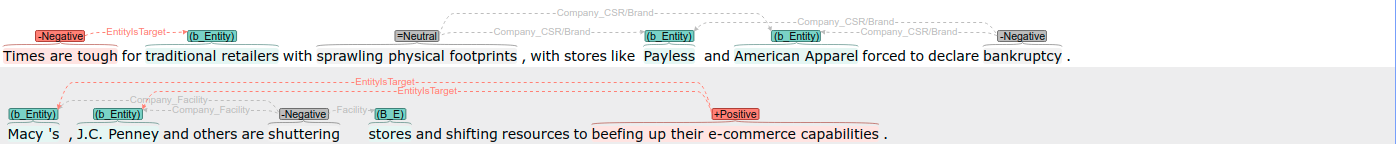
\includegraphics[width=\textwidth]{img/amzn00s9-10 negative event example.png}
    \caption*{$\rightarrow$ \textbf{Sentiment Expression}: ``Times are tough'' is a negative Sentiment Expression, ``beefing up their e-commerce capabilities'' is a Positive Sentiment Expression, ``sprawling physical footprints'' is a neutral Sentiment Expression as a pre-existing Event annotation, ``bankruptcy'' is a negative Sentiment Expressions  as a pre-existing Event annotation, ``shuttering'' is a negative Sentiment Expression as a pre-existing Event annotation.}
    \label{fig:se_ex2}
\end{figure}

\noindent
\textcolor{BrickRed}{NOTE: \textbf{Relevancy} of sentiment expressions: since we are primarily interested in company-specific investor sentiment you should only annotate new \textbf{sentiment expressions that are relevant to a company}. Sentiment expressions about companies, company-specific assets, reports or metrics, and people, infrastructure or subsidiaries related to a company are relevant should be annotated. Irrelevant background information about products, locations or other details that do not \textbf{affect an investors opinion of a company} should not be annotated.}

\subsection{Sentiment Polarity}
\label{sec:polaritydefinition}
Sentiment Expressions always have a positive, negative or neutral Polarity.
Polarity is the emotional opinion value of the Sentiment Expression.
Positive polarity signals an optimistic, desirable, pleasant or favourable disposition, while Negative polarity signals pessimistic, undesirable, or unpleasant attitudes.

For our definition of common-sense investor sentiment, positive polarity are Sentiment Expressions that express a positive attitude towards a business entity directly or are indirectly good for an investor looking to invest in that business entity. Positive polarity Sentiment Expressions then signal all things that increase the likelihood of return on profit when investing in the target business entity.
Negative polarity does the opposite: negative polarity Sentiment Expressions decrease the likelihood of a return on profit when investing in the target.

Besides positive and negative polarity, we also annotate Neutral polarity making three polarity values in total:

\begin{enumerate}[label=\alph*), leftmargin=*] % insert figure here and explain in more detail
    \item \textbf{Positive}: an event, opinion or situation that increases the likelihood of a return on investment.
    Positive Sentiment Expressions directly or indirectly improve the attitude of a potential investor towards the target.
    \item \textbf{Negative}: an event, opinion or situation that increases the likelihood of a loss on investment.
    Negative Sentiment Expressions directly or indirectly diminish the attitude of a potential investor towards the target.
    \item \textbf{Neutral}: an event, opinion or situation has no clear positive or negative polarity.
    This happens when a) it is unclear how the Sentiment Expression affects a potential investor's attitude or b) the annotator cannot identify a clearly positive or negative polarity.
    When doubting between Positive/Negative and Neutral sentiment, annotators should prefer to assign Positive/Negative.
    % \item \textbf{Conflict}: the sentiment of an event, opinion or situation depends on the point of view of the reader or is highly debatable.
    % Personal preferences, political bias, or sentiment highly dependent on context or perspectives outside of the article are typical cases.
    % Do not confuse this with Neutral sentiment: there should be a clear conflict of point of view, not an unclear sentiment.
     % TODO Make this a double tagging rule instead of CONFLICT and DISCUSS in DIFFICULT CASES SECTION
\end{enumerate}

\begin{figure}[h]
\captionsetup[subfigure]{labelformat=empty}
\begin{subfloat}
    \centering
    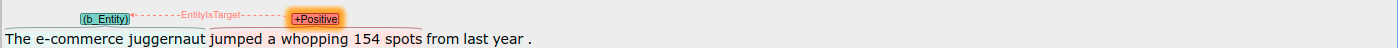
\includegraphics[width=\textwidth]{img/amzn00-s04 pos example.png}
    \caption*{$\rightarrow$ \textbf{Positive}: New Sentiment Expression ``jumped a whopping 154 spots [in ranking]'' is Positive for the e-commerce giant Amazon.}
\end{subfloat}

\begin{subfloat}
    \centering
    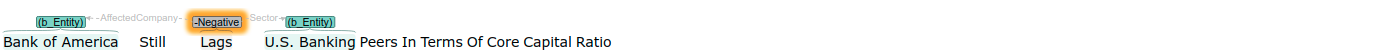
\includegraphics[width=\textwidth]{img/bac02s01 negative example.png}
    \caption*{$\rightarrow$ \textbf{Negative}: Pre-existing Event annotation ``Lags'' is Negative for ``Bank of America''.}
\end{subfloat}

\begin{subfloat}
    \centering
    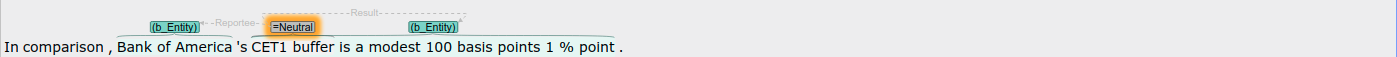
\includegraphics[width=\textwidth]{img/bac02s04 neutral example.png}
    \caption*{$\rightarrow$ \textbf{Neutral}: Pre-existing Event annotation ``CET1 Buffer'' is Neutral for ``Bank of America'' as it is not clearly bad or good.}
\end{subfloat}

% % TODO FIND A BETTER CONFLICT EXAMPLE BECAUSE THIS ONE IS NOT IT
% \begin{subfloat}
%     \centering
%     
\includegraphics[width=\textwidth]{img/amzn00s01 conflict example.png}
%     \caption*{$\rightarrow$ \textbf{Conflict}: Pre-existing Event annotation ``Closing in'' is good for ``Amazon'' and ``Alibaba'', but bad for ``Walmart''. Due to this conflict inherent in the event we annotate Conflict polarity.}
% \end{subfloat}
\end{figure}

\begin{wrapfigure}[4]{R}{0.3\textwidth}
    \centering
    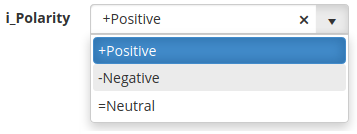
\includegraphics[width=0.3\textwidth]{img/polarityui.png}
    \vspace{-10pt}
    \label{fig:polarityui}
\end{wrapfigure}

\noindent
\textcolor{Blue}{Annotate Polarity in the WebAnno interface:
1) Select the Sentiment Expression or pre-existing Event in the annotation panel by double-clicking.
2) Select \texttt{Positive}, \texttt{Negative}, or \texttt{Neutral} from the drop-down menu next to \texttt{f\_Polarity} in the side panel.}

\subsection{Sentiment Uncertainty}
\label{sec:uncertaintydefinition}
Most sentiment expressions are asserted by the news article author as lacking any uncertainty.
However, some Sentiment Expressions have a degree of uncertainty: these are represented by the author as probable, possible or likely sentiment expressions and improbably, impossible or unlikely sentiment expressions.
The author indicates it is a \textbf{possibility, probability or likelihood that the event takes place or does not take place}.
The Uncertainty label also includes cases in which the author signals that he does not know the certainty level or does not commit to asserting a fact.

Uncertainty can be realized by uncertainty markers such as verbal auxiliaries (must, may), adverbials (probably, possibly, presumably), and adjectives (likely, possible).
In many cases, uncertainty will be conveyed by verbs near the sentiment expression: "seem", "think", "want", "wish", "hope", "speculate", "propose", \annexe{The company \uline{wants} to \anntrg{fire} its factory line workforce.}

\begin{figure}[h]
    \centering
    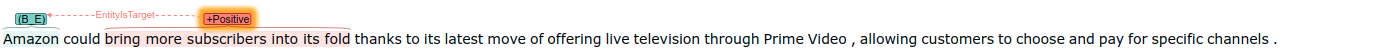
\includegraphics[width=\textwidth]{img/amzn04s31 uncertain example.png}
    \caption*{$\rightarrow$ \textbf{Uncertain}: Sentiment Expression ``bring more subscribers into its fold'' is uncertain due to the auxiliary verb ``could''.}
    \label{fig:unc_ex1}
\end{figure}

\noindent
\textcolor{BrickRed}{NOTE: Uncertainty only has to be annotated on new Sentiment Expressions. Pre-existing Events already have Uncertainty annotated by previous annotators.}\\

\begin{wrapfigure}{R}{0.2\textwidth}
    \centering
    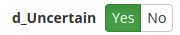
\includegraphics[width=0.2\textwidth]{img/uncertainui.png}
    \label{fig:uncertainui}
\end{wrapfigure}

\noindent
\textcolor{Blue}{Annotate Uncertainty in the WebAnno interface:
1) Select the Sentiment Expression in the annotation panel by double-clicking.
2) Click the toggle in the side panel next to \texttt{e\_Uncertain} if the sentiment has Uncertainty otherwise do nothing. The toggle should turn from red \texttt{No} to green \texttt{Yes}.}


\subsection{Sentiment Negation}
\label{sec:negationdefinition}

Usually, the sentiment expressed by the Sentiment Expression is affirmative and asserted, meaning that it is being represented as being true or as something that will happen/has happened.
However, a Sentiment Expression can also be negated in its context.
\textbf{A negative form expresses the falsity of the opinion, event or situation expressed}.
It communicates the opposite meaning of the opinion, event or situation.
This is typically realized by ``not'', ``-n't'', ``no'', ``noone'', ``nowhere'' or other negative forms.\\

\noindent
\textcolor{BrickRed}{NOTE: The negation word should not be tagged as part of the Sentiment Expression.
Because of this, the Polarity of the sentiment should be opposite of its meaning in the full negated context:}\\

\begin{figure}[h]
    \centering
    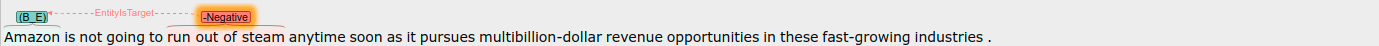
\includegraphics[width=\textwidth]{img/amzn04s34 negated negative sentiment.png}
    \caption*{$\rightarrow$ \textbf{Negated}: we annotate ``run out of steam'' and not ``is not going to run out of steam'' as the Sentiment Expression: we do not include the negation word ``not''. While the meaning of the whole sentence is Positive, ``run out of steam'' is tagged as Negative because the phrase on its own is Negative.}
    \label{fig:neg_ex1}
\end{figure}

\begin{figure}[h]
    \centering
    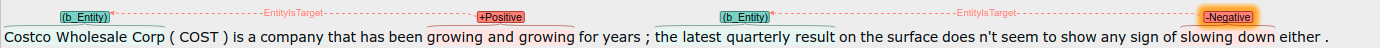
\includegraphics[width=\textwidth]{img/cost02s02 new sentiment negative uncertain.png}
    \caption*{$\rightarrow$ \textbf{Negated + Uncertain}: ``slowing down'' is negated by ``doesn't'' and uncertainty is added by ``seem''. While the meaning of the whole sentence is Positive, ``slowing down'' is tagged as Negative because on its own without the negation of ``doesn't'' it signals Negative polarity.}
    \label{fig:neg_ex2}
\end{figure}

\noindent
\textcolor{BrickRed}{NOTE: Negation only has to be annotated on new Sentiment Expressions. Pre-existing Events already have Negation annotated by previous annotators.}\\

\begin{wrapfigure}{l}{0.2\textwidth}
    \centering
    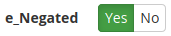
\includegraphics[width=0.2\textwidth]{img/negationui.png}
    \label{fig:negationui}
\end{wrapfigure}

\noindent
\textcolor{Blue}{Annotate Negation in the WebAnno interface:
1) Select the Sentiment Expression in the annotation panel by double-clicking.
2) Click the toggle next to \texttt{e\_Negated} if the sentiment is negated otherwise do nothing. The toggle should turn from red No to green Yes.}

\section{Events (Pre-existing annotation)}
\label{sec:eventdefinition}
When you open a document in the WebAnno interface, pre-existing annotations will be present in the text that were made in a previous annotation task.
You will add your own sentiment annotations on top of these annotations.
There are two pre-existing annotation categories: Events and Entities.
Here we discuss Events briefly:\\
\eventcolor Event annotation with label \texttt{a\_Event} and label \texttt{d\_EventPart} for unconnected words that are part of the event.

\begin{figure}[!htb]
    \centering
    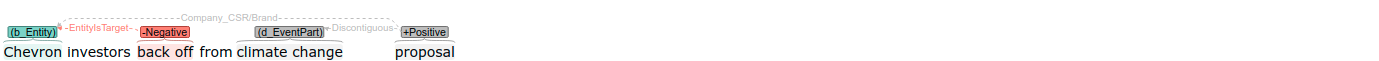
\includegraphics[width=\textwidth]{img/cvx00s01 event part.png}
    \caption*{$\rightarrow$ \textbf{Split Event+EventPart}: ``climate change proposal'' is split in two labels but should be read as one Event.}
\end{figure}

Events denote real-world actions, changes and situations which are relevant to economic news.
These events come from a prescribed set of 18 categories such as ``Investment'', ``Dividend'', ``Security Value'', ``Mergers \& Acquisitions'', etc. 
You should ignore the types of these events, however note that potentially relevant Events not belonging to these 18 types were not annotated.
This means that you will have to pay attention to relevant news events that invoke sentiment and annotate them as new Sentiment Expressions.\\

\noindent
\textcolor{BrickRed}{NOTE: Often pre-existing Event annotations will not include all words that capture the full sentiment.
In that case, we simply assign the polarity on the event as if it was part of a full Sentiment Expression.}
\begin{figure}[h]
    \centering
    
\includegraphics[width=\textwidth]{img/fb03 incomplemte event trigger example.png}
    \caption*{$\rightarrow$ \textbf{Event}: ``terrorism'' is a pre-existing Event annotation. While the full Sentiment Expression would be ``cracking down on terrorism'', indicating Positive opinion, you only have to assign the polarity on the pre-existing Event, not on the whole phrase.}
\end{figure}

Annotators assign all pre-existing Events a polarity value of Positive, Negative, or Neutral taking into account the definition of events above.
Annotators should take into account the \textbf{whole context of the event when determining the event polarity}.
This means that the framing of the event and its participants are important. However, an \textbf{exception are Negated events which should ignore the negation context} when annotating polarity in the same manner as new Sentiment Expressions. Negation has already been tagged on these Events as a pre-existing annotation.\\

\noindent
\textcolor{BrickRed}{NOTE: When multiple Events are annotated in the same location. Do not forget to determine polarity for all Events taking into account the different Entities involved in the different Events. If they have the same Entities, annotate the same polarity on all events.}
\begin{figure}[h]
    \centering
    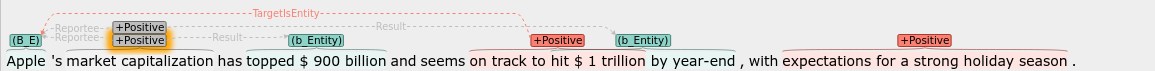
\includegraphics[width=\textwidth]{img/aapl15 s04 two events in same place.png}
    \caption*{$\rightarrow$ \textbf{Event}: ``market capitalization'' has two pre-existing Event annotations. The first links to the Entity ``topped \$ 900 billion'', indicating Positive opinion. The second event links to Entity ``hit \$ 1 trillion by year-end'' which is also Positive. Polarity for both events is annotated.}
\end{figure}

\section{Entities (Pre-existing annotation)}
\label{sec:entitydefinition}
\entitycolor Entity annotations with label \texttt{b\_Entity}.
    
These are the central participants involved in the event.
Entities play a typical role in the Event to which they are linked.
They are often companies, persons, assets or monetary amounts.
This role label is visible in the annotation interface on the link, but should be ignored for our purposes.
The existing entity annotations can be realized as pronouns (``it'', ``its'', ``he(r)''. ``they'', ``we'') or non-specific descriptions (``the company'', ``the bank'', ``the tech giant'').
If you annotate new entities as targets (cf. \ref{sec:entitydefinition}) you should not annotate pronouns but the nearest specific mention of the entity.

You will also make new Entity annotations when they are the target of a Sentiment Expression.

\begin{figure}[h]
    \centering
    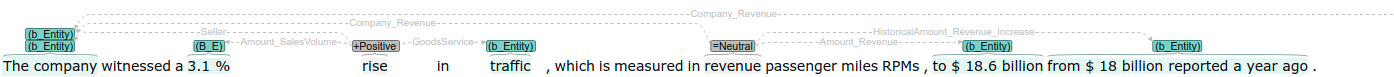
\includegraphics[width=\textwidth]{img/aal00s03 entities example.png}
    \caption*{$\rightarrow$ \textbf{Entity}: Several \entitycolor pre-existing Entity annotations as participants in the Event annotations.}
    \label{fig:ent_ex1}
\end{figure}

\section{Target}
\label{sec:targetdefinition}
The target of a sentiment is the company, person, product, asset, entity, etc. about which the sentiment is expressed.
A person always expresses an opinion about some topic and that topic is the target.
The target is the entity about which a potential investor forms his opinion.
One Sentiment Expression can have multiple targets and all targets should be tagged.

\noindent
In our annotation task we have three categories of targets:
\begin{enumerate}[label=\alph*), leftmargin=*]
    \item \textbf{New target entity}: the target entity is expressed by words on which NO Entity or Event annotation exists.
    \begin{figure}[!htb]
    \centering
    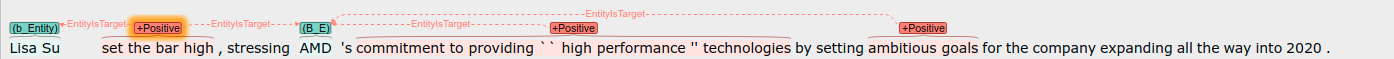
\includegraphics[width=\textwidth]{img/amd02s08 new entity.png}
    \caption*{$\rightarrow$ This sentence had no pre-existing annotations. New target Entity annotations must be made for ``Lisa Su'' target of Sentiment Expression ``set the bar high'', ``AMD'' target of ``commitment to providing...'' and ``ambitious goals''.}
\end{figure}

    \item \textbf{Existing Entity}: the target entity is expressed by words on which a \entitycolor Entity annotation exists.
    \begin{figure}[!htb]
    \centering
    
\includegraphics[width=\textwidth]{img/aal02s11 entity .png}
    \caption*{$\rightarrow$ Sentiment Expression ``on time'' targets pre-existing Entity ``AA''.}
\end{figure}
    
    \item \textbf{Existing Event}: the target is an event on which a \eventcolor Event annotation exists.
    \begin{figure}[!htb]
    \centering
    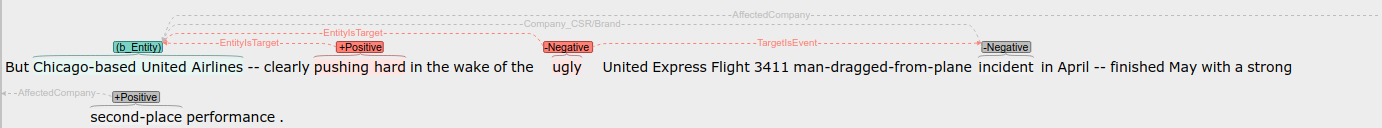
\includegraphics[width=\textwidth]{img/aal02s06 entity target example.png}
    \caption*{$\rightarrow$ ``ugly'' has two targets: pre-existing Event ``incident'' and pre-existing Entity ``Chicago-based United Airlines''.}
\end{figure}
\end{enumerate}

You will have to annotate new targets and link the Sentiment Expression to existing Event or Entity targets.
Keep the \textbf{word sequence of New target annotations as small as possible} to capture the core meaning of the target.

\newpage
\noindent
\textcolor{BrickRed}{NOTE: \textbf{Target-dependent polarity}: The \textbf{sentiment polarity of an expression changes depending on the target}.
This usually happens when a contrasting comparison is made between two companies.
In that case, annotate two different Sentiment Expressions with different polarity and targets in the same place.\\
An existing Event can also have different polarity for different participants.
In this case, annotate the Event itself as Neutral because its Polarity is ambiguous and make new Sentiment Expressions exactly on top of the existing Event expression with the Polarity corresponding to each Target.}

\begin{figure}[!ht]
    \centering
    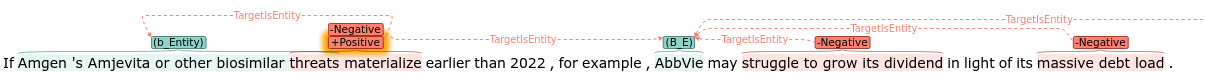
\includegraphics[width=\textwidth]{img/abbv07 s31 target dependent new sentiment example.png}
    \caption*{$\rightarrow$ \textbf{Target-dependent polarity double tagging}: New Sentiment Expression ``threats materialized'' is positive for the target ``Amgen's Amjevita or other biosimilar threats'', but negative for ``AbbVie'' so we annotate one positive and one negative Sentiment Expression in the same place.}
\end{figure}

\begin{figure}[!ht]
    \centering
    
\includegraphics[width=\textwidth]{img/amz00 s01 target dependent polarity double tagging on event.png}
    \caption*{$\rightarrow$ \textbf{Target-dependent polarity double with existing Event}: Existing Event ``Closing in'' is tagged as ``Neutral'' because the event itself is ambiguous. 
    Two new Sentiment Expressions are made exactly in the same place as ``Closing in'': One Positive for targets ``Amazon'' and ``Alibaba''and another Negative for ``Walmart''.}
\end{figure}


% ISSUES TO BE RESOLVED: if one event combines a positive or negative effect on different participants
% Possible solution:
% - Annotate Conflict as polarity
% - 


\chapter{Workflow}
\label{chapter/workflow}
\begin{steps}[leftmargin=*]
    % \item Read the document once.
    % If you have issues understanding something we encourage you to ask the supervisor or look up any terms/companies/acronyms.
    
    \item \label{step:start} Read the \textbf{next sentence}.
    If \eventcolor \texttt{a\_Event} annotations already exist: go to step \ref{step:forevent}
    If no pre-existing \texttt{a\_Event} are present: go to step \ref{step:annotatesentiment}
    
    \item \label{step:forevent} Decide \hyperlink{sec:polaritydefinition}{\textbf{Polarity}} for each \hyperlink{sec:eventdefinition}{pre-existing \texttt{a\_Event}}.
    \begin{enumerate}[label=\alph*), leftmargin=*] \label{step:polarity}% insert figure here and explain in more detail
        \item \texttt{Positive}: the event/sentiment is mostly positive.
        \item \texttt{Negative}: the event/sentiment is mostly negative.
        \item \texttt{Neutral}: the event/sentiment has no clear positive or negative connotation.
        \item \texttt{Conflict}: the event/sentiment depends on the point-of-view.
    \end{enumerate}
    \textcolor{OliveGreen}{Click on each \eventcolor \texttt{a\_Event} annotation and choose Polarity using the \texttt{i\_Polarity} drop-down menu in the side panel.}
    
    \item \label{step:annotatesentiment} Annotate all \hyperlink{sec:sentimentexpressiondefinition}{\textbf{Sentiment Expressions}} as the \textbf{smallest possible number of words} denoting \hyperlink{sec:sentimentdef}{investor sentiment} in the sentence. % 
    \textit{Which words express an opinion or could affect an investors opinion?}\\
    \textcolor{OliveGreen}{Select \texttt{1\_Sentiment} in the Layer drop-down menu (top-right side panel), drag the mouse across the words that express the sentiment in the Annotation panel. \footnotesize{Selection of the annotation layer fails sometimes. To fix: Unselect the current annotation with the \texttt{Clear} button, select a different layer than \texttt{1\_Sentiment} and next re-select \texttt{1\_Sentiment}.}}\\
    \textcolor{BrickRed}{NOTE: Sentiment words that are part of/overlap with a pre-existing Event/Entity but do not correspond fully in meaning $\rightarrow$ Annotate a new overlapping Sentiment Expression.}\\
    % NOTE: Sentiment words overlap with existing event: If the sentiment words intensify or change the opinion of the smaller event annotation, annotate the sentiment expression separately including the event words so that they overlap.
    
    
    \item \label{step:decidetargets} Select each \texttt{1\_Sentiment} and annotate all the \hyperlink{sec:targetdefinition}{\textbf{Targets}}.
    \textit{What is the opinion about?}.\\
    One Sentiment Expression can have \textbf{multiple targets}: make sure links are drawn to each target.\\
    \textcolor{OliveGreen}{While the \sentimentcolor \texttt{1\_Sentiment} annotation is selected (glowing outline)}:
        \begin{enumerate}[label=\alph*), leftmargin=*]
            \item \label{step:linkentity} Target is \hyperlink{sec:entitydefinition}{a pre-existing \entitycolor Entity} $\rightarrow$ \textbf{Link Entity}:\\
            \textcolor{OliveGreen}{
            Click on the \texttt{Click to activate} field next to ``EntityIsTarget'' in the side panel.
            Click on the \entitycolor \texttt{b\_Entity} in the Annotation panel.
            }
            \item \label{step:linkevent} Target is \hyperlink{sec:eventdefinition}{a pre-existing \eventcolor Event} $\rightarrow$ \textbf{Link Event}:\\
            \textcolor{OliveGreen}{
            Click on the \texttt{Click to activate} field next to "EventIsTarget" in the side panel.
            Click on the \eventcolor \texttt{a\_Event} in the Annotation panel.
            }
            \item \label{step:newtarget} Target on words without an existing annotation $\rightarrow$ \textbf{Create and Link a new target}:\\
            \textcolor{OliveGreen}{
            Click on the \texttt{Click to activate} field next to "EventIsTarget" in the side panel.
            Drag your mouse across the smallest possible amount of words indicating the entity in the Annotation panel.
            }
            \item \label{step:multiple} Multiple targets $\rightarrow$ \textbf{Add more than one target}:\\
            \textcolor{OliveGreen}{
            Click on \texttt{Select Role} in the drop-down menu under ``EntityIsTarget'' (if target is existing or new Entity) or ``EventIsTarget'' (if target is existing Event) and click the \texttt{Add} button. Proceed as in the previous options.
            }
        \end{enumerate}
        
        \item Decide \hyperlink{sec:polaritydefinition}{\textbf{Polarity}}, cf. step \ref{step:polarity}.\\
        \textcolor{BrickRed}{NOTE: Sometimes the sentiment polarity is different depending on the target. In these cases, we make a new sentiment annotation and link Targets to which the sentiment polarity corresponds.}
        
        \item Decide \hyperlink{sec:uncertaintydefinition}{\textbf{Uncertainty}}: \textit{Is the sentiment expression presented as being uncertain?}\\
        \textcolor{OliveGreen}{
        Toggle \texttt{d\_Uncertain} from red ``No'' to green ``Yes'' in the side panel.
        }
        
        \item Decide \hyperlink{sec:negationdefinition}\textbf{Negation}: \textit{Is the sentiment expression negated?}\\
        \textcolor{OliveGreen}{
        Toggle \texttt{e\_Negated} from red ``No'' to green ``Yes'' in the side panel.
        }
        
    \item Continue on to the next sentence; go to step \ref{step:start}
    
\end{steps}

\begin{figure}[!htb]
    \centering
    \caption*{Workflow overview chart}
    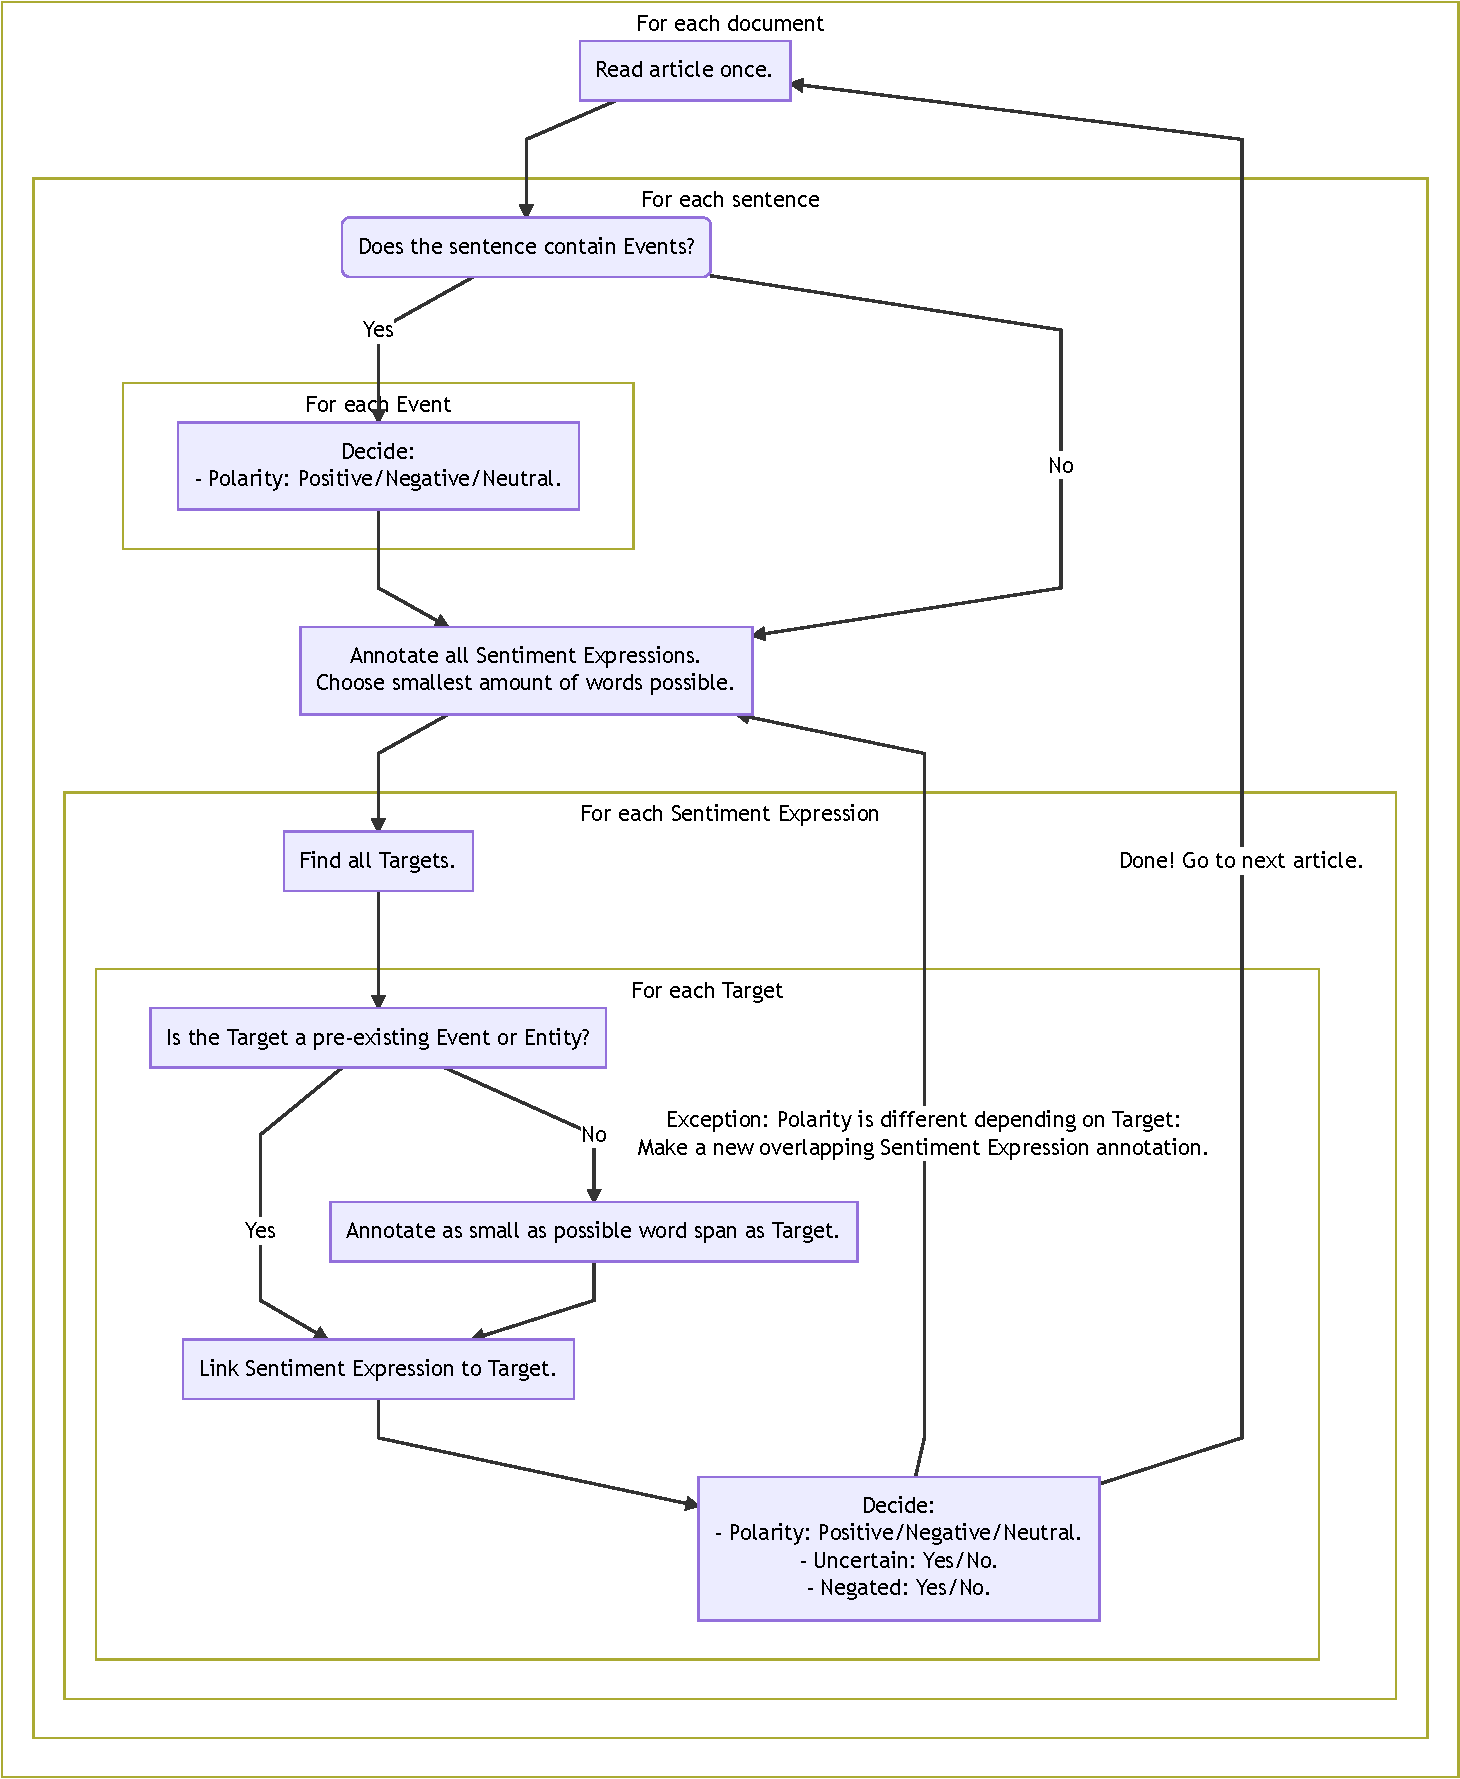
\includegraphics[width=\textwidth]{img/workflow-diagram-cropped.pdf}
\end{figure}

\chapter{Annotation Interface}
\label{chapter/interface}
\begin{figure}[!htb]
    \centering
    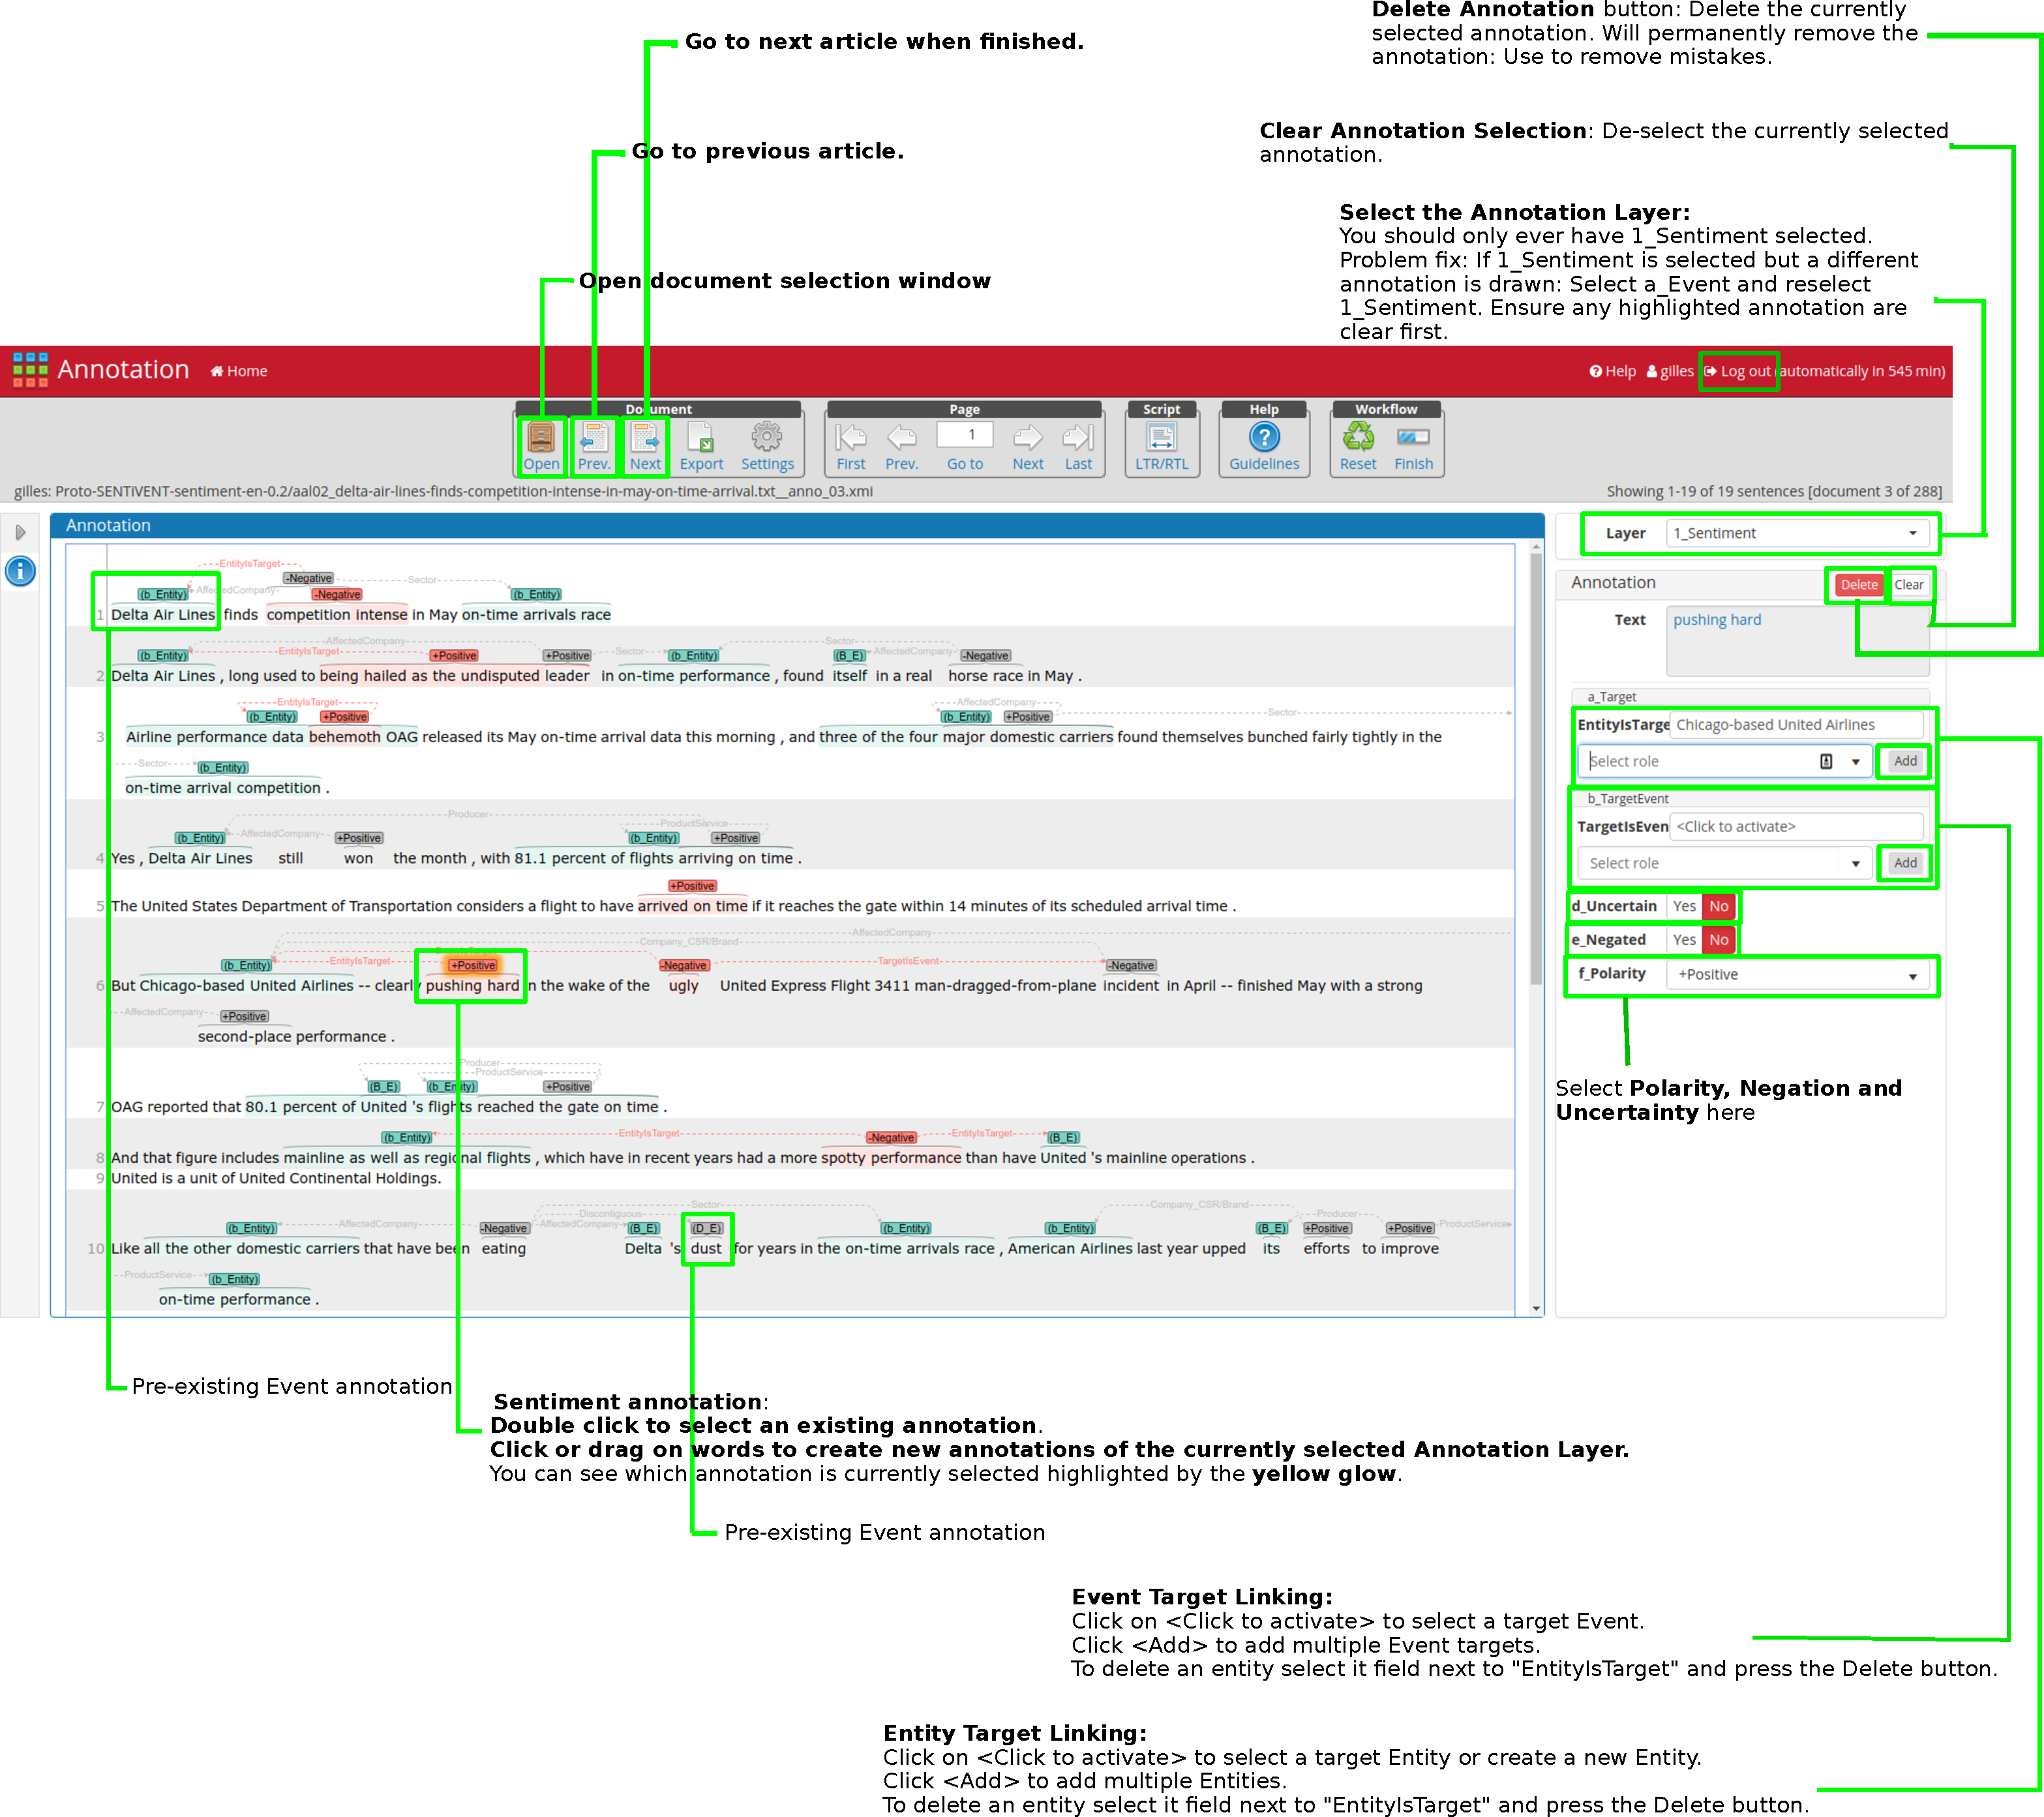
\includegraphics[width=\textwidth]{img/webanno-interface.pdf}
    \caption{WebAnno interface with primary functions explained.}
\end{figure}

\noindent
Basic actions:
\begin{itemize}[leftmargin=*]
    \item Double left mouse click an existing annotation bubble to select the annotation. The selected annotation has a glowing outline.
    \item Left mouse click + drag over a word or multiple words will create a new annotation of the type selected in the Layer drop-down menu (top-right side panel).
    \item To de-select a selected annotation: press the Clear button in the side-panel top-right.
    \item To remove an annotation (in case of a mistake): press the Delete button in the side-panel top-right.
    \
\end{itemize}

\tagged{full}{
\chapter{Sentiment design choices}
\label{chapter/sentiment}
\section{What is sentiment}

Sentiment is positive or negative opinion that is expressed in text.

% Common-sense investor sentiment
Point of view: investor sentiment: someone looking to invest in the company, product or entity mentioned in a 
Investing is the act of allocating funds to an asset or committing capital to an endeavor (a business, project, real estate, etc.), with the expectation of generating an income or profit. Positive investor sentiment thus entails the opinion that the investee is worth allocating funds too with the expectation it will generate wealth over a period of time.
Negative investor sentimen entails the opposite: there is the expectation that a loss will be made and the invested funds will not be recuperated. There is some financial risk associated with the sentiment target.

We collected a corpus of company-specific economic news articles.
These articles are largely written with the express purpose of informing the wider public as potential stock market investors about recent events pertaining to a company, industry, or market.

\section{Related work dataset comparison}
\subsection{Differences between SENTiVENT and EventDNA}
% Differences in event conceptualization
\textbf{Event annotation differences:} The EventDNA project \cite{colruyt2019leveraging} also aims to relate events to sentiment as ``polar facts'' in news text.
While the goal is similar, the definition and annotation of events are different between our SENTiVENT event annotations \cite{jacobs2020sentiventeventguidelines} and EventDNA annotations \cite{Colruyt2019}:

\begin{enumerate}[wide, labelwidth=!, nolistsep, label=\alph*)]
\item \textbf{General vs. economic news domain}:
EventDNA focusses on general news reporting, while SENTiVENT focusses on company-specific business news.
EventDNA uses the Rich ERE event typology for general news text, while SENTiVENT developed its own company-specific typology for economic events.

\item \textbf{Entity annotation}:
EventDNA annotates entities separately in line with Rich ERE while SENTiVENT does not.
In SENTiVENT only entities that participate in events as arguments are tagged.

\item \textbf{Annotation of event triggers}:
EventDNA does not annotate event triggers as as-small-as-possible lexical units as SENTiVENT but annotates whole clauses, nominal constructions and infinitive constructions.
The event triggers of EventDNA span a large amount of continuous tokens corresponding to clausal units including arguments, while SENTiVENT triggers are smaller lexical units excluding arguments.
EventDNA's approach greatly simplifies annotation of event triggers and recovers lexical head units using automatic syntactic dependency parsing \cite{colruyt2019leveraging}.
Hence, SENTiVENT/ACE/ERE-like triggers and EventDNA's triggers can by mapped for multi-task experiments using dependency parsers with custom rules in the clausal > lexical direction and inversely use automatic clause boundary detection \cite{sharma2016clause} in the lexical > clausal direction.

\item \textbf{Event attributes}: There are minor differences in how SENTiVENT and EventDNA handle event attributes such as realis, modality, tense, prominence.
Realis and modality attributes between SENTiVENT and EventDNA are comparably binary: negated events are tagged as such and modality is also either asserted or other.
EventDNA includes a Tense for capturing time information and Event Prominence which annotates if the event is the main event/news peg in the news article attribute while SENTiVENT does not.\\
\end{enumerate}

\textbf{Sentiment annotation differences:} 

\begin{enumerate}[wide, labelwidth=!, nolistsep, label=\alph*)]
\item \textbf{General common-sense vs. investor sentiment}: EventDNA attempts to capture general common-sense event sentiment AKA polar facts: the prototypical sentiment related to events by the general public. SENTiVENT attempts to capture prototypical investor sentiment on company-specific events. % explain more

\item \textbf{Sentiment on entities}: EventDNA tags all entities in a text, including those outside of events, and annotates their prototypical sentiment polarity. SENTiVENT only on entities that are event arguments leading to less entities with sentiment.
\end{enumerate}

\subsection{SENTiVENT vs. Rich ERE}
As explained in \ref{historyeventextract} Rich ERE is the latest iteration of a line of research including ACE and Light ERE.  % todo write section and use correct label
We will focus mainly on Rich ERE as we largely based our event annotations on these guidelines.

% pasted from sentivent-doctoraatsthesis/chapt-data/chapt-data.tex
Our event conceptualization is highly similar to the Rich ERE annotation scheme with the major difference that event arguments are not restricted by entity type.
The largest divergence from Rich ERE is the fact that ERE annotates a set of pre-defined entities before the event annotation phase.
Entities and relations are not annotated in our work.
We do not tag entities separately, i.e. any text span that describes a relevant event argument within the extent is tagged.
Rich ERE in contrast requires the more strict Argument Entities which are entity classes within the scope/extent of the current event of a particular pre-determined type.
We do maintain the ERE distinction between two argument types: Participant arguments and filler arguments.
In Rich ERE, filler arguments are non-predefined arguments that are not pre-annotated and are also not limited to event mention scope. i.e. they can be annotated from anywhere in the document.
Event argument definitions are hence not restricted by entity types.
This make the task more similar to the semantic frame annotation practices as in FrameNet \cite[Chapter~3]{ruppenhofer2010framenet} which are lexicographically motivated: lexical units (i.e. word token-spans) that convey a core meaning of the event arguments are annotated unrestricted by entity type or syntax.

Another major difference from Rich ERE is how we operationalize factuality:
ERE events have one feature Realis with three values: .
Our events have two features Polarity and Modality.

Rules that define the extent (i.e., token-span length and lexical units) are also taken from Rich ERE.
These rules determine how long spans should be and help annotators in ambiguous cases.
In comparison with other event conceptualizations such as \cite{sprugnoli2017} names this the Event Nugget conceptualization in DEFT Rich ERE: unlike ACE or Light ERE, Rich ERE allows for discontinuous and multi-token spans but are discouraged.

The event typology for Rich ERE is meant to be for knowledge-base population from general text domain.
ACE/ERE event types betray an interest in governmental socio-political tracking with military, political related event types such as Conflict, Contact, Movement, Transaction, Justice events etc.
% TODO add number of event types and check genres in TAC KBP Rich ERE annotations NEWS mainly?
Our work focuses on domain-specific events in the company-specific economic news genre.
This naturally leads to a different, more specific event typology.

\subsection{SENTiVENT vs. SentiFM}
SentiFM is the predecessor to the SENTiVENT project and also aims to assign economic sentiment in business news.
The focus of SentiFM lies on processing of implicit sentiment and events are tagged as a type of entity in text.

Events in SentiFM are defined by 10 types.
The event triggers are loosely defined and are allowed to be discontinuous.
This leads to event triggers that typically correspond to clausal units.
No event arguments are tagged except for one relation which is the same for all events type: the company to which the event relates.
No realis, tense, factuality, negation attributes are tagged.

Sentiment-wise SentiFM provides highly detailed fine-grained annotations.
SentiFM thus presents a dataset in which sentiment and event are not directly linked in annotation.

\section{What are aspect}


}

\tagged{full}{
\nocite{*}
\printbibliography[heading=bibintoc]
}

\end{document}
